\section{Retângulo}

\begin{frame}[fragile]{Representação de retângulos}

    \begin{itemize}
        \item Um retângulo é um quadrilátero com os quatro ângulos internos iguais 
        \pause

        \item Assim, cada ângulo tem 90\textdegree, pois a soma dos ângulos internos de um 
            quadrilátero é igual a 360\textdegree
        \pause

        \item Os pares de lados opostos (paralelos) de um retângulo são denominados base e
            altura
        \pause

        \item Deste modo, um retângulo pode ser representado de duas formas: a primeira delas é 
            através da medida de sua base e de sua altura
    \end{itemize}
        \pause

    \inputcode{cpp}{codes/rectangle.cpp}

\end{frame}

\begin{frame}[fragile]{Representação de retângulos}

    \begin{itemize}
        \item A segunda maneira é representar o triângulo através das coordenadas de 
            vértices opostos
        \pause

        \item Na matemática o mais comum é utilizar o canto inferior esquerdo e o canto superior 
            direito
        \pause

        \item Na computação gráfica é o contrário: são utilizados o canto superior esquerdo e o 
            canto inferior direito
        \pause

        \item A vantagem desta representação é que ela permite a fácil dedução da base e da 
            altura, e dá flexibilidade na implementação de algoritmos que envolvem retângulos

    \end{itemize}

\end{frame}

\begin{frame}[fragile]{Exemplo de representação de retângulo por vértices}
    \inputcode{cpp}{codes/rect.cpp}
\end{frame}

\begin{frame}[fragile]{Perímetro e área}

    \begin{itemize}
        \item O perímetro de um retângulo é igual ao dobro da soma de suas dimensões 
            (base e altura)
        \pause

        \item A área é igual ao produto destas dimensões
    \end{itemize}
        \pause

    \inputcode{cpp}{codes/area.cpp}
\end{frame}

\begin{frame}[fragile]{Quadrados}

    \begin{itemize}
        \item Um quadrado é um retângulo com lados iguais
        \pause

        \item Não há necessidade de implementar uma estrutura à parte para os quadrados, 
            uma vez que todos os resultados válidos para os retângulos permanecem válidos para os 
            quadrados
        \pause

        \item Contudo, um quadrado pode ser representado por apenas uma dimensão (lado), de modo
            que instâncias de quadrados podem ocupar apenas a metade da memória necessária
            para um retângulo
        \pause

        \item Embora a relação ``um quadrado é um retângulo"\ seja verdadeira, ela não precisa
            ser implementada por herança
        \pause

        \item Ou se usa composição ou não se especializa o quadrado, usando o próprio retângulo
    \end{itemize}

\end{frame}

\begin{frame}[fragile]{Interseção entre retângulos}

    \begin{itemize}
        \item A interseção entre dois retângulos cujos lados sejam paralelos aos eixos ordenados pode ser determinada a partir da 
            interseção entre dos intervalos referentes às projeções dos retângulos nos eixos 
            $x$ e $y$
        \pause

        \item A interseção pode ser vazia (não há interseção), um segmento de reta ou um retângulo
        \pause

        \item Os últimos dois cenários podem ser diferenciados através da área do retângulo 
            resultante, onde área igual a zero significa um segmento de reta
    \end{itemize}
        \pause

    \begin{figure}
        \centering

        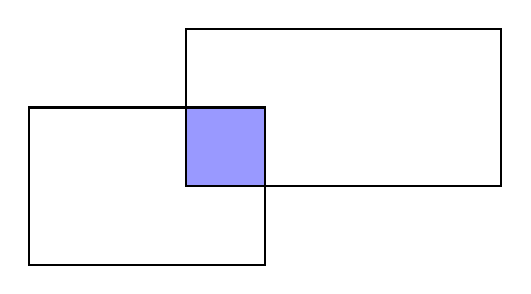
\begin{tikzpicture}
            \coordinate (A) at (0, 0);
            \coordinate (B) at (3, 2);
            \coordinate (C) at (2, 1);
            \coordinate (D) at (6, 3);

            \coordinate (X) at (2, 1);
            \coordinate (Y) at (3, 2);

            \fill[color=blue!40] (X) rectangle (Y);

            \draw[thick] (A) rectangle (B);
            \draw[thick] (C) rectangle (D);

        \end{tikzpicture}
    \end{figure}
\end{frame}

\begin{frame}[fragile]{Implementação da interseção entre retângulos}
    \inputsnippet{cpp}{1}{17}{codes/intersection.cpp}
\end{frame}

\begin{frame}[fragile]{Implementação da interseção entre retângulos}
    \inputsnippet{cpp}{19}{42}{codes/intersection.cpp}
\end{frame}
